This benchmark originates in \cite{dohu03}. It is also carried out in \cite{bepo10}.
It considers the advection of a product-cosine hill
in a prescribed velocity field. The initial temperature is:
\begin{equation}
T_0(x,y)=
\left\{
\begin{array}{cc}
\frac{1}{4}
\left(1+\cos \pi\frac{x-x_c}{\sigma}\right)
\left(1+\cos \pi\frac{y-y_c}{\sigma}\right)
& \text{if } (x-x_c)^2+(y-y_c)^2\leq \sigma^2 \\
0 & \text{otherwise}
\end{array}
\right.
\end{equation}
The boundary conditions are $T(x,y)=0$ on all four sides of the unit square domain. In what follows we set $x_c=y_c=1/6$ and $\sigma=0.2$.  The velocity field is analytically prescribed: $\vec\upnu=(-(y-y_c),+(x-x_c))$.

In what follows we test the time integration scheme by setting $\alpha_T=1$ (fully implicit formulation), $\alpha=0$ (fully explicit formulation) and $\alpha_T=1/2$ (Crank-Nicolson).  
The timestep is set to $\delta t=2\pi/200$. The density and heat capacity values are set to 1. 
We monitor the minimum and maximum value of the temperature field, as well as the total thermal energy $E_T$ in the system during the 200 time steps ($2\pi$ rotation of the cone):
\[
E_T=\int_\Omega \rho_0 c_p T dV = \int_\Omega T dV = |\Omega| \langle T \rangle 
\qquad
\text{where}
\qquad
\langle T \rangle = \frac{1}{|\Omega|} \int_\Omega T dV
\]
The time evolution of the temperature with the Crank-Nicolson algorithm is shown hereunder:
\begin{center}
a)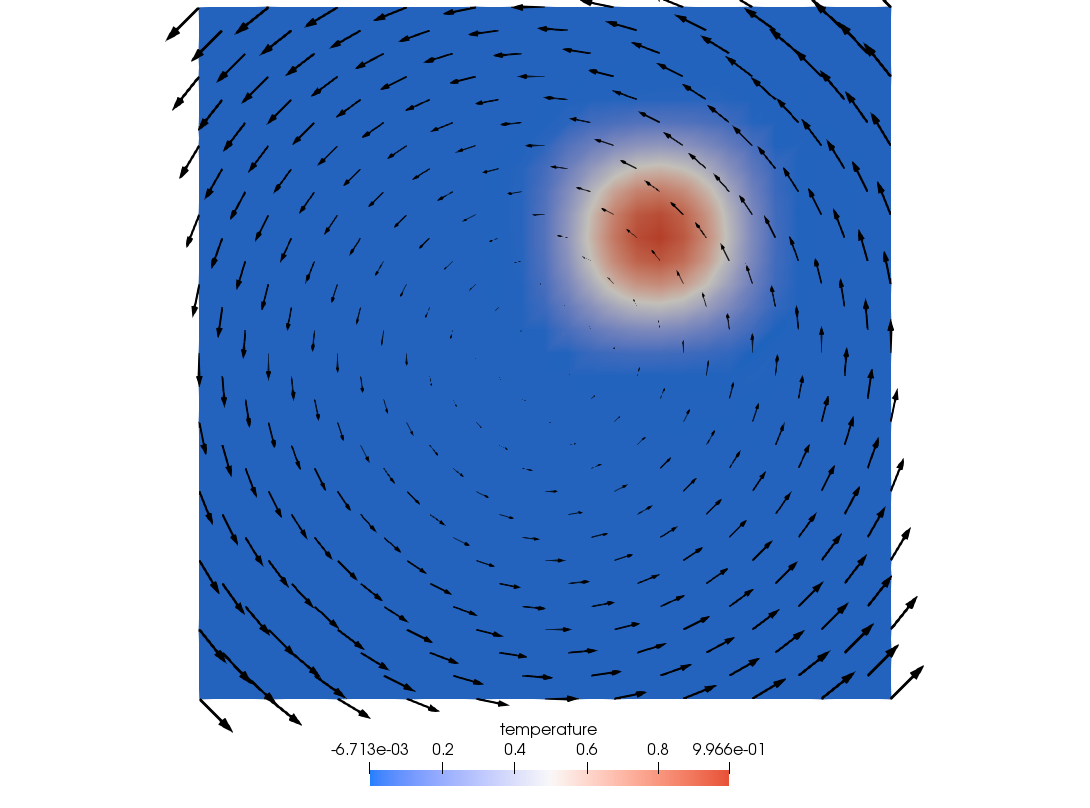
\includegraphics[width=4.8cm]{python_codes/fieldstone_43/images/crni/velfield}
b)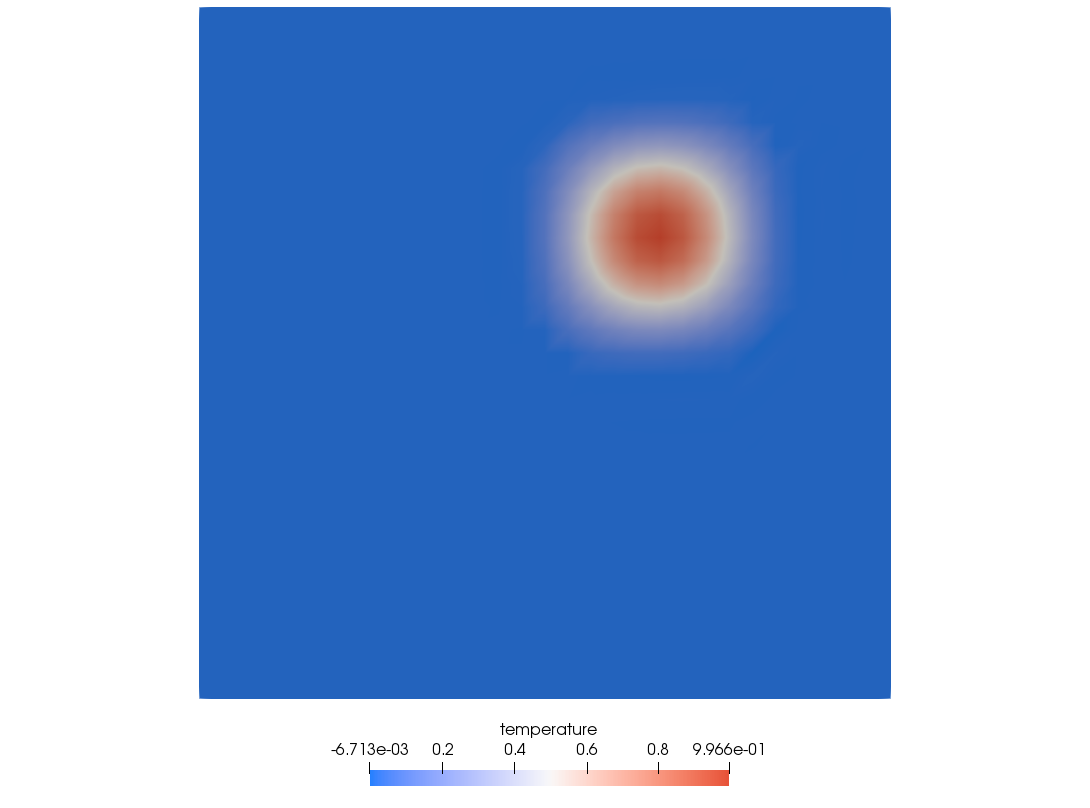
\includegraphics[width=4.8cm]{python_codes/fieldstone_43/images/crni/crnitemp0000}
c)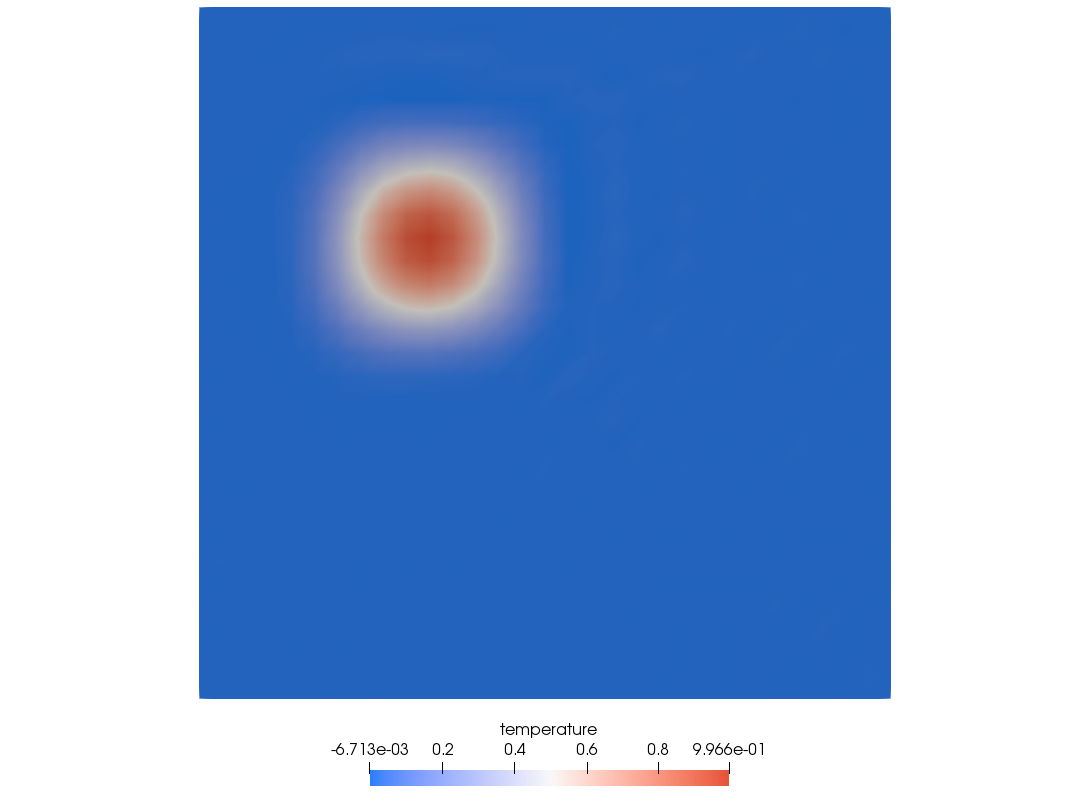
\includegraphics[width=4.8cm]{python_codes/fieldstone_43/images/crni/crnitemp0050}\\
d)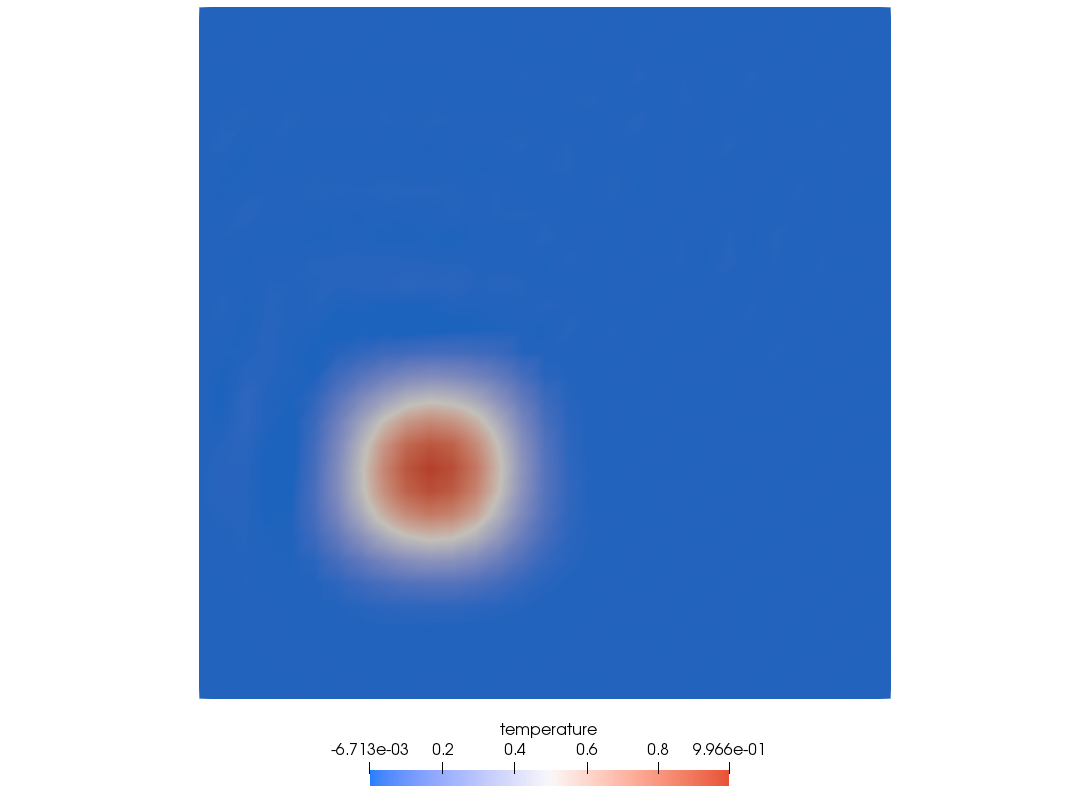
\includegraphics[width=4.8cm]{python_codes/fieldstone_43/images/crni/crnitemp0100}
e)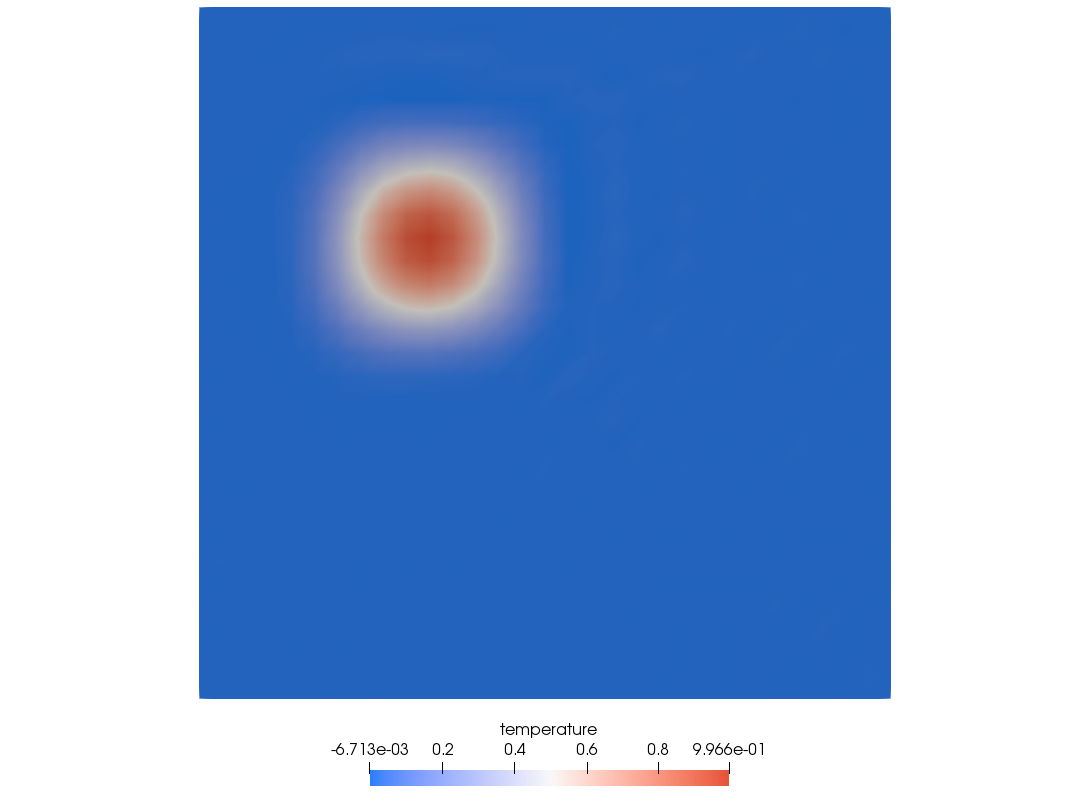
\includegraphics[width=4.8cm]{python_codes/fieldstone_43/images/crni/crnitemp0050}
f)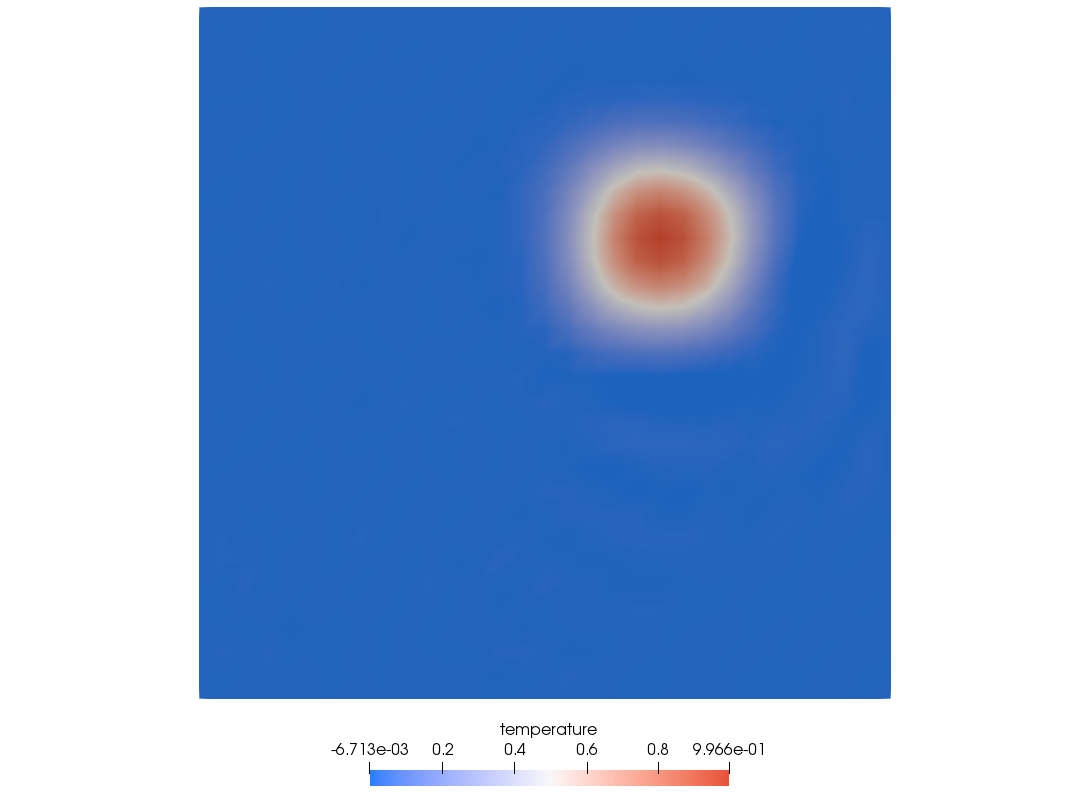
\includegraphics[width=4.8cm]{python_codes/fieldstone_43/images/crni/crnitemp0199}\\
{\small a) Velocity field and initial temperature; b,c,d,e,f) Temperature field at timesteps 0,50,100,150,199.} 
\end{center}
Turning now to the statistics, we plot $\min(T)$, $\max(T)$ and $E_T$ as a function of time:
\begin{center}
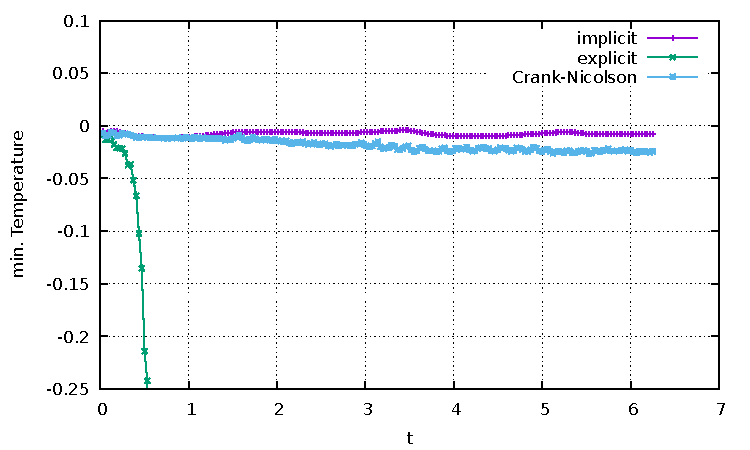
\includegraphics[width=5cm]{python_codes/fieldstone_43/images/Tmin.pdf}
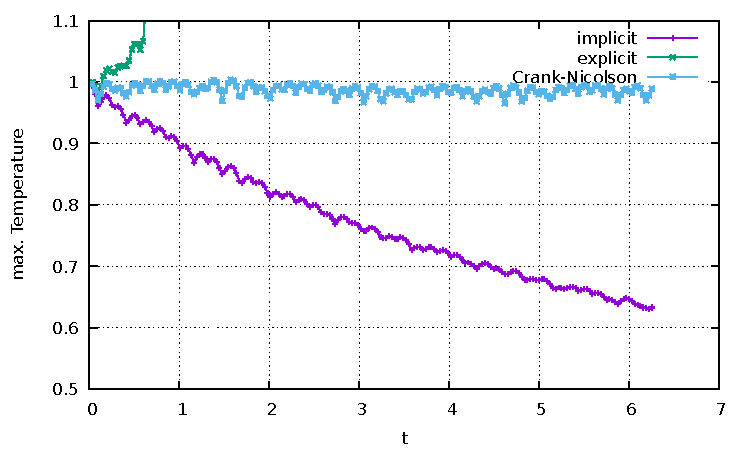
\includegraphics[width=5cm]{python_codes/fieldstone_43/images/Tmax.pdf}
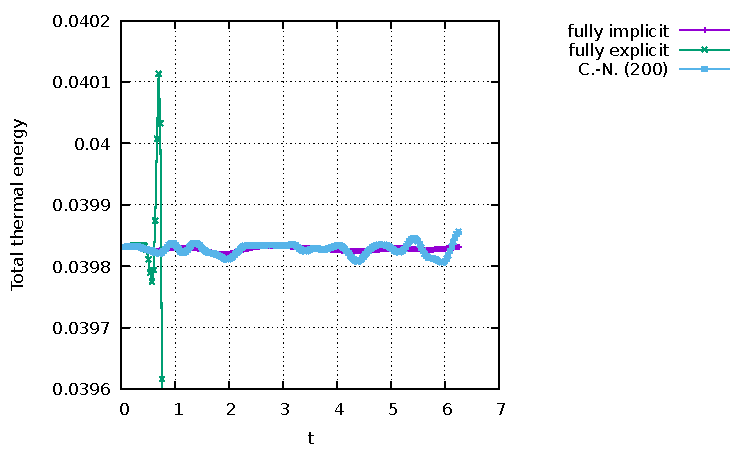
\includegraphics[width=5cm]{python_codes/fieldstone_43/images/ET.pdf}\\
{\small Time evolution of the min and max temperature and the total energy}
\end{center}
The conclusions are clear: the explicit method diverges quickly and is unusable. The fully implicit and Crank-Nicolson 
method yield similar energy conservation but the fully-implicit showcases a clear loss in maximum temperature as shown in the following figure:
\begin{center}
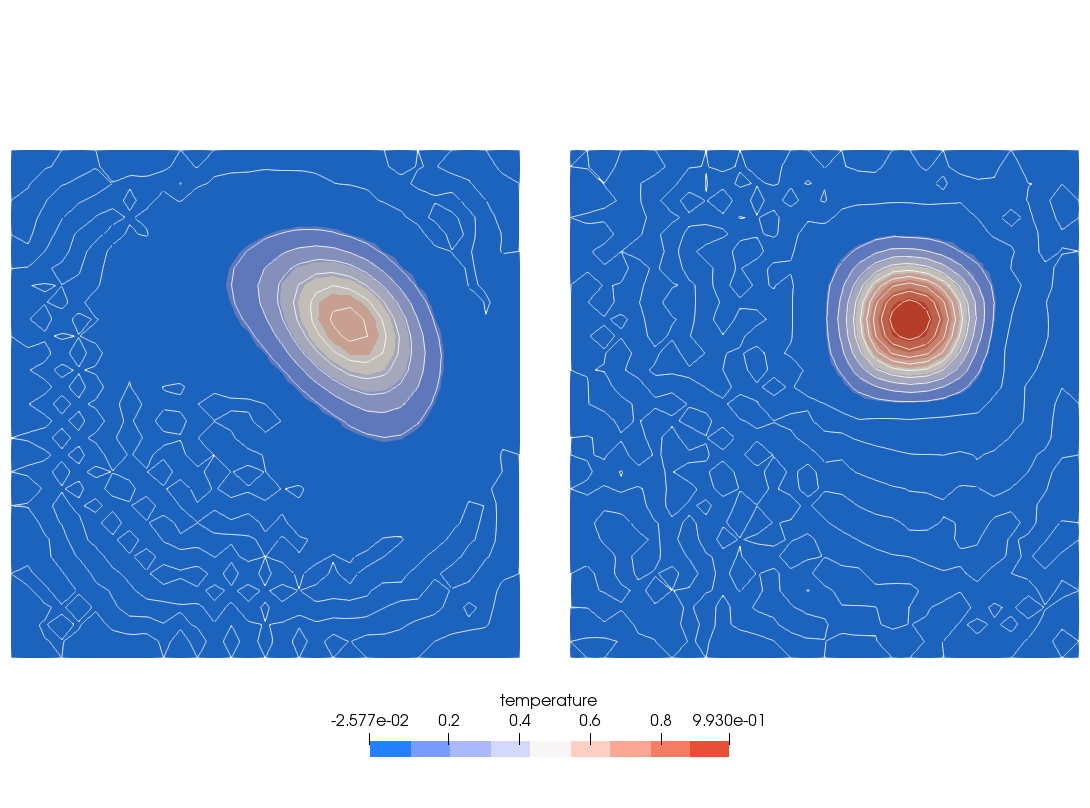
\includegraphics[width=15cm]{python_codes/fieldstone_43/images/temp}\\
{\small Temperature field after a full rotation with isocontours every 0.1 value.\\ Left: Fully-implicit; Right: Crank-Nicolson}
\end{center}

Finally we can run the experiment (still a $2\pi$ rotation) 
with three different time steps ($\delta t=2\pi/30,2\pi/60,2\pi/120$) 
and we recover very similar results to those presented in \cite{dohu03}:

\begin{center}
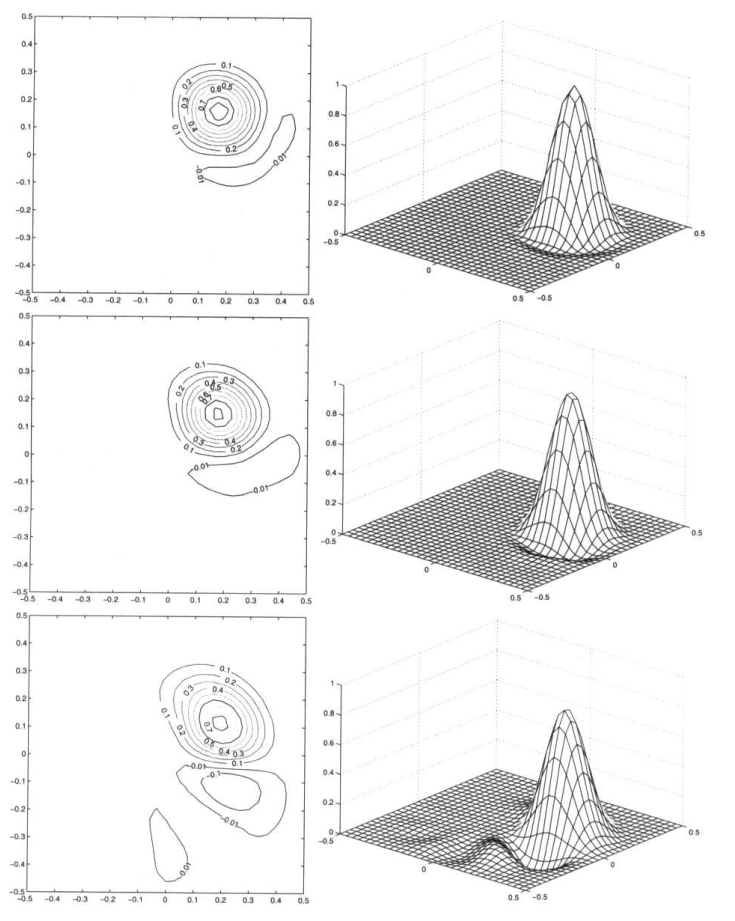
\includegraphics[height=8cm]{python_codes/fieldstone_43/images/dohu03}
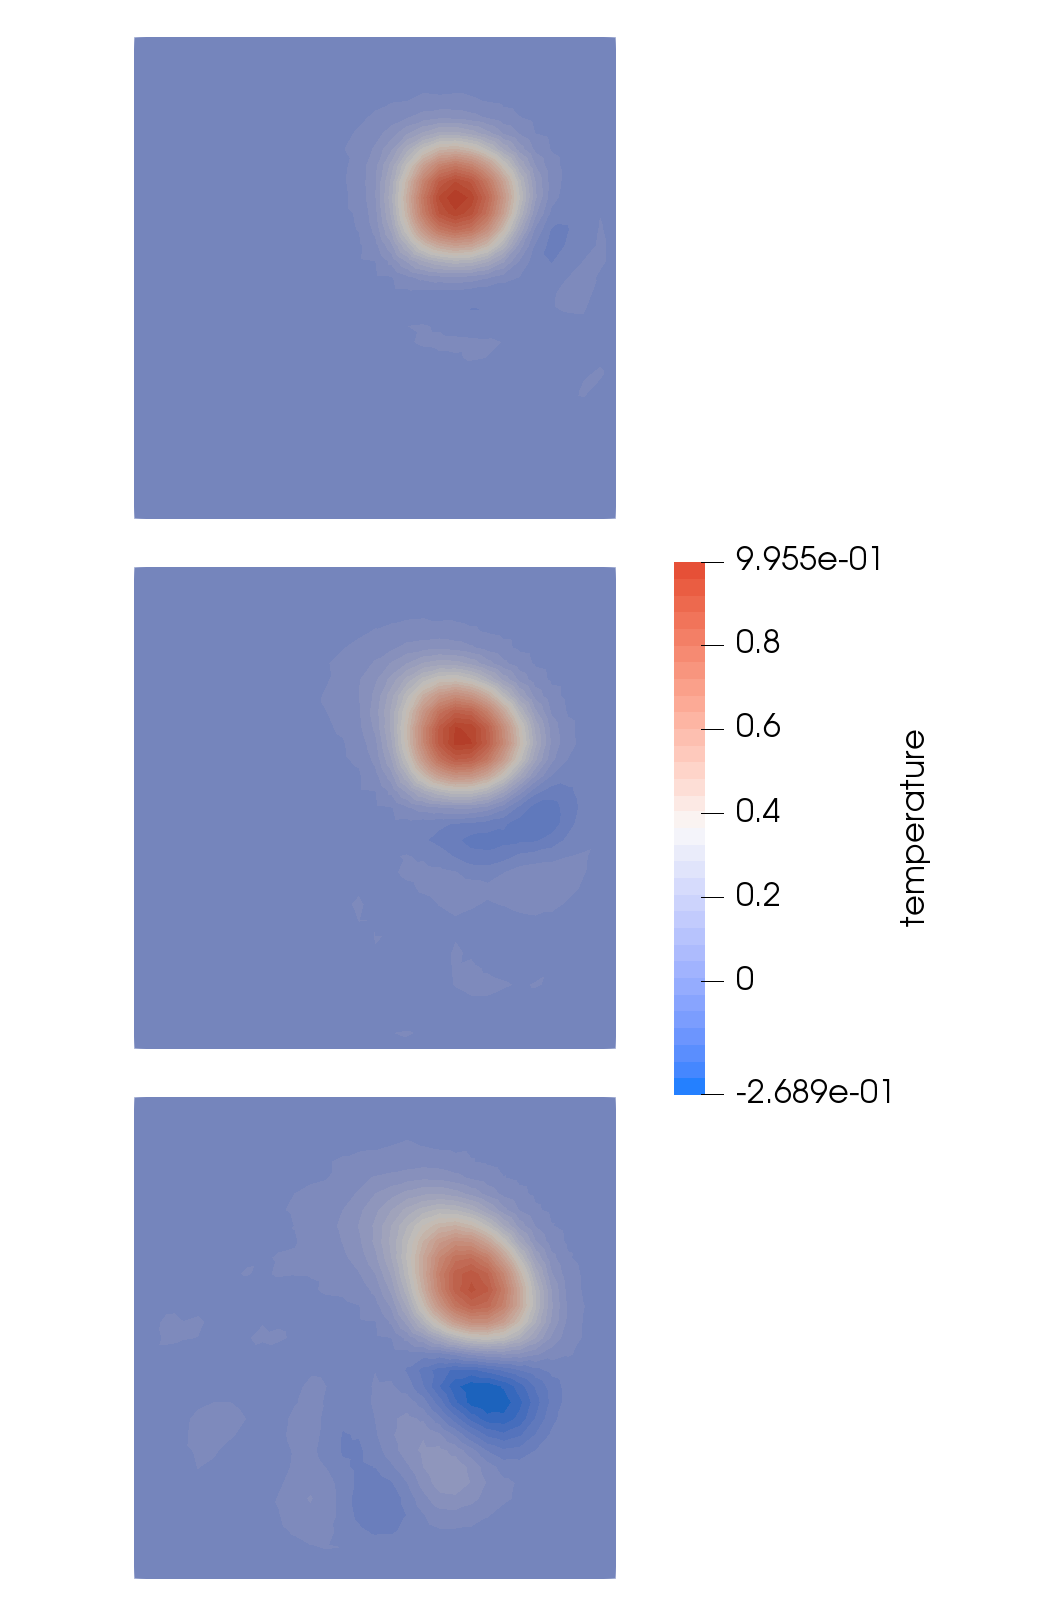
\includegraphics[height=8cm]{python_codes/fieldstone_43/images/temps_30_60_120}\\
{\small From top to bottom: $\delta t=2\pi/120,2\pi/60,2\pi/30$ with Crank-Nicolson. Left panel is taken from donea \& Huerta \cite{dohu03}}
\end{center}

\begin{center}
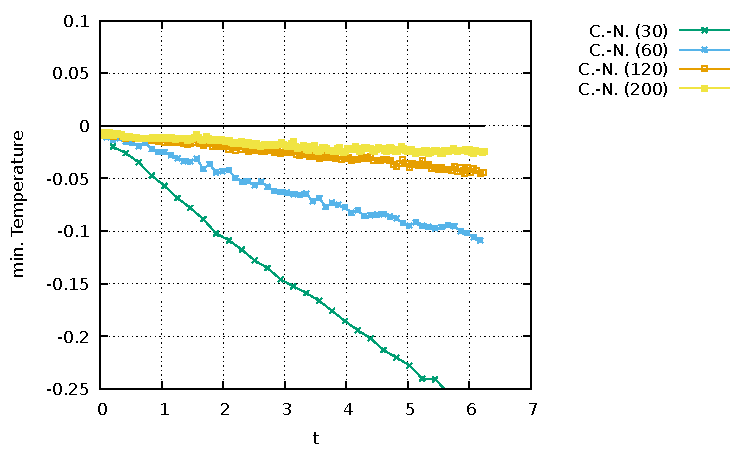
\includegraphics[width=5cm]{python_codes/fieldstone_43/images/Tmin_CN.pdf}
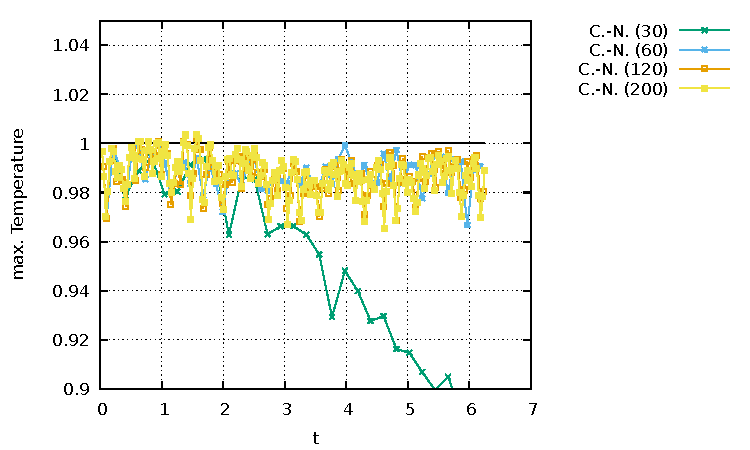
\includegraphics[width=5cm]{python_codes/fieldstone_43/images/Tmax_CN.pdf}
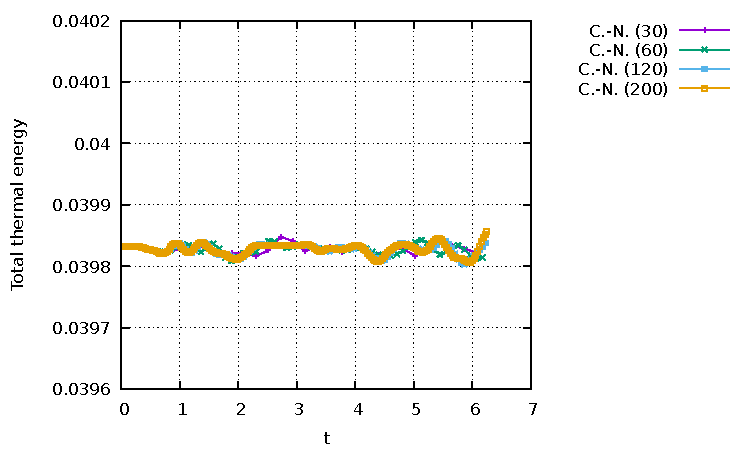
\includegraphics[width=5cm]{python_codes/fieldstone_43/images/ET_CN.pdf}\\
{\small Time evolution of the min and max temperature and the total energy obtained with the Crank-Nicolson algorithm for 4 values of the timestep as indicated by the number between parenthesis.}
\end{center}


\begin{center}
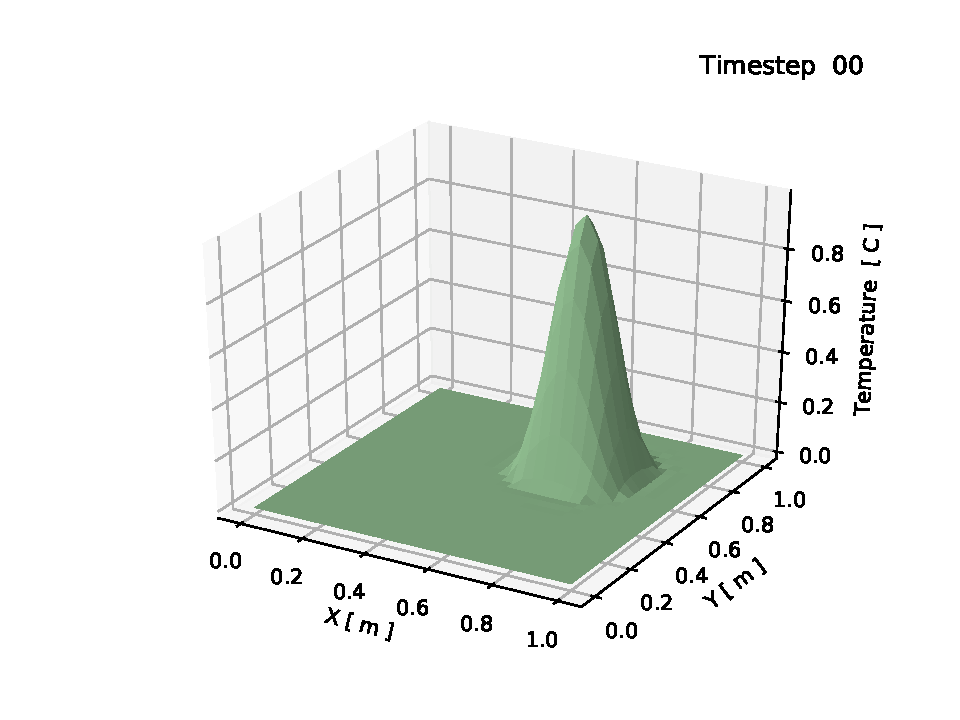
\includegraphics[width=3cm]{python_codes/fieldstone_43/images/solution_0000.pdf}
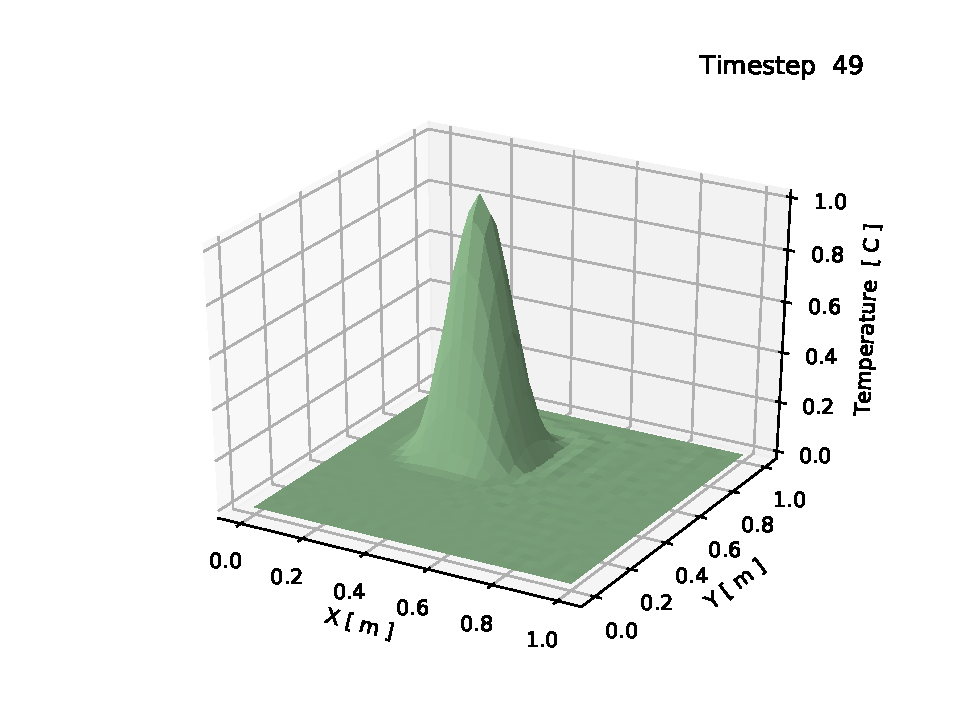
\includegraphics[width=3cm]{python_codes/fieldstone_43/images/solution_0049.pdf}
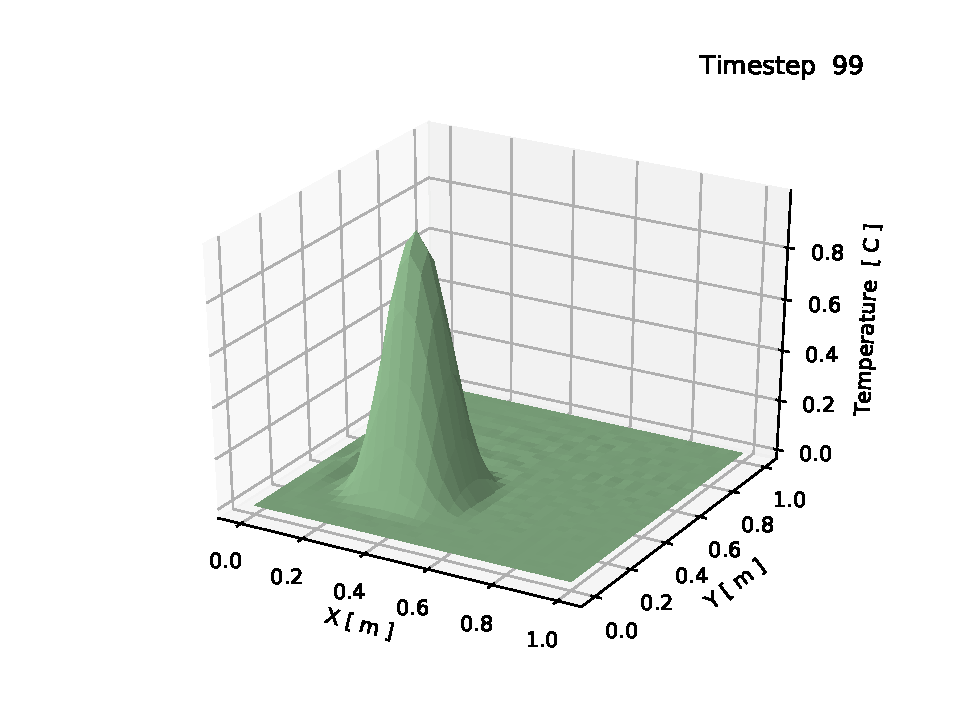
\includegraphics[width=3cm]{python_codes/fieldstone_43/images/solution_0099.pdf}
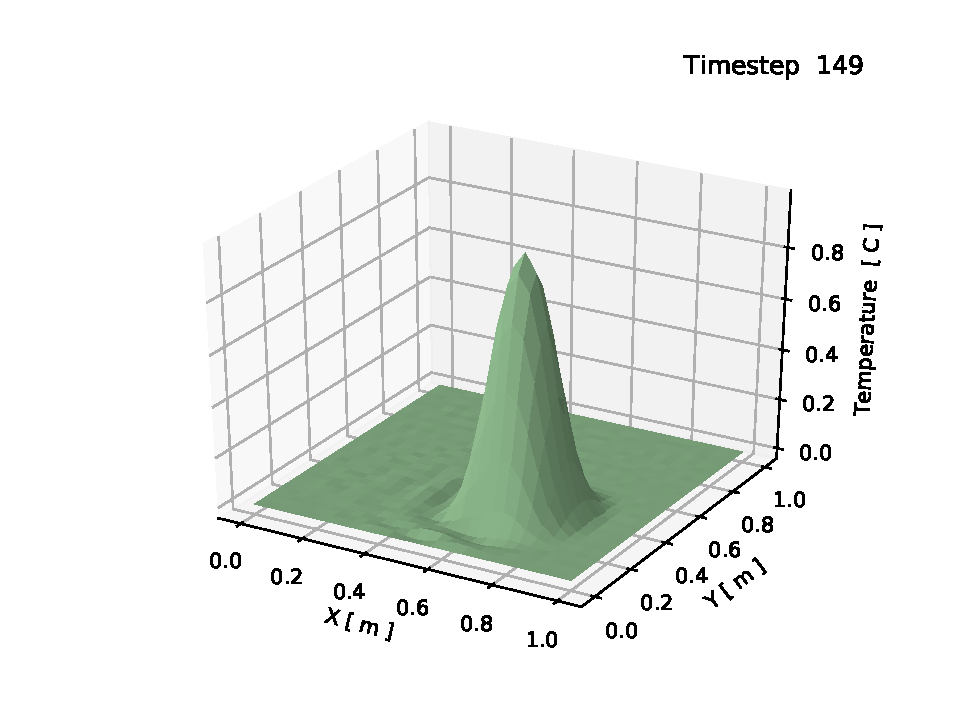
\includegraphics[width=3cm]{python_codes/fieldstone_43/images/solution_0149.pdf}
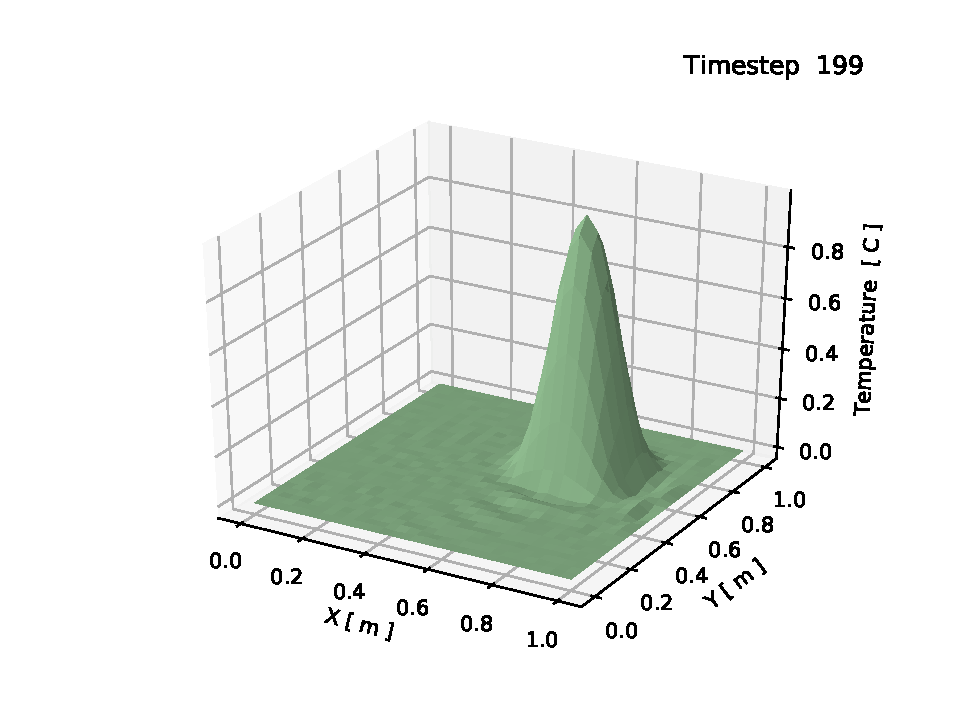
\includegraphics[width=3cm]{python_codes/fieldstone_43/images/solution_0199.pdf}\\
{\small Time evolution of the temperature field for $\delta t=2\pi/200$ with Crank-Nicolson.}
\end{center}

